\documentclass[a4paper,12pt]{article}
\usepackage[margin=1in]{geometry}

\usepackage[T2A]{fontenc}			% кодировка
\usepackage[utf8]{inputenc}			% кодировка исходного текста
\usepackage[english,russian]{babel}	% локализация и переносы
\usepackage{graphicx}                % Математика
\usepackage{amsmath,amsfonts,amssymb,amsthm,mathtools} 
\usepackage{mathtext}
\usepackage[T2A]{fontenc}
\usepackage[utf8]{inputenc}

\usepackage{wasysym}

%Заговолок
\author{Бичина Марина 
группа Б04-005 1 курса ФЭФМ}
\title{}
\date{}


\begin{document} % начало документа

\begin{center}
\begin{Large}
{Бичина Марина, Карташов Константин Б04-005, Лабораторная работа №. 5.1.1 <<Экспериментальная проверка уравнения Эйнштейна для фотоэффекта и определение постоянной Планка>>}
\end{Large}
\end{center}
\paragraph{Цель работы:} 
\begin{enumerate}
\itemsep0em
\item Исследовать зависимость фототока от 
\begin{enumerate}
\itemsep0em
\item величины задерживающего потенциала
\item частоты падающего излучения
\end{enumerate}
\item вычислить постоянную Планка
\end{enumerate}

\section{Теоретическая справка}
\paragraph{}
\textbf{Фотоэффект} -- явление испускания электронов фотокатодом, облучаемым светом. Это явление хорошо объясняется фотонной теорией света: взаимодействие монохроматического света с веществом можно описывать как взаимодействие с веществом частиц, называемых фотонами, которые обладают энергией $ \hbar \omega $ и импульсом $ \hbar\omega/c $. При столкновении фотона с электроном фотокатода энергия фотона полностью передается электрону, и фотон прекращает свое существование. Энергетический баланс этого взаимодействия для вылетающих электронов описывается уравнением
	
\begin{equation}
\hbar \omega = E_{max} + W
\label{e:energy_balance}
\end{equation}
	
\begin{figure}[h!]
\centering
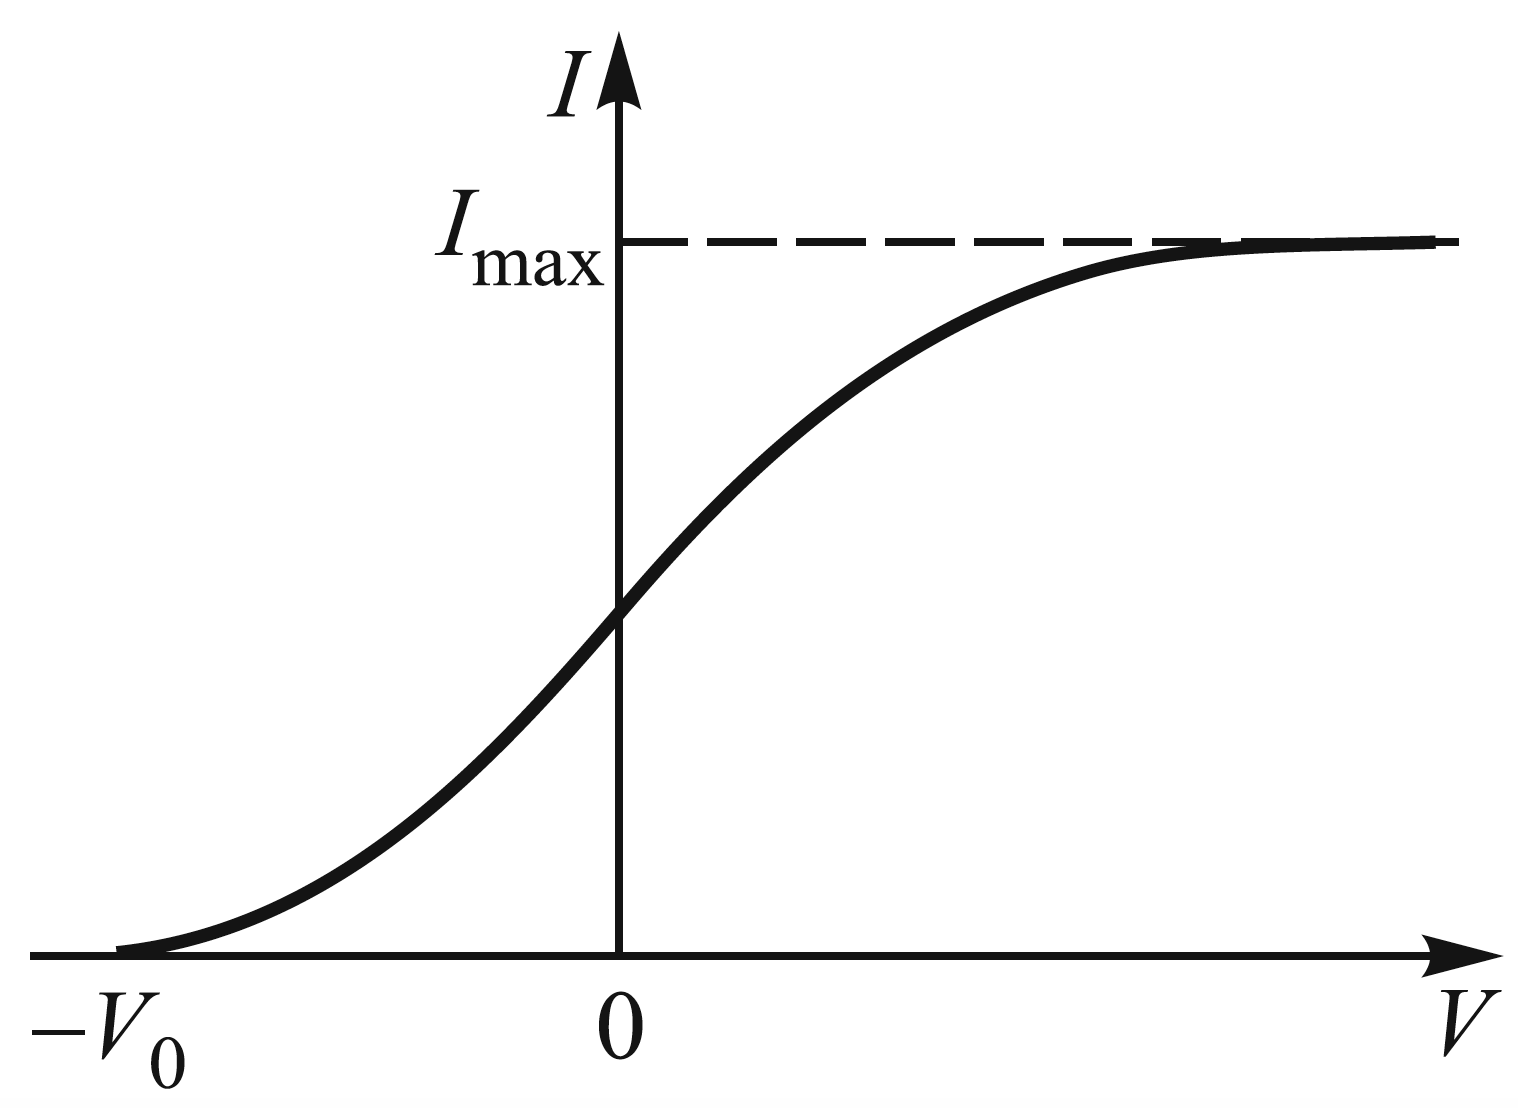
\includegraphics[scale=0.3]{I(V)}
\caption{Зависимость фототока от напряжения на аноде фотоэлемента}
\label{fig:iv_theory}
\end{figure}
	
Где $ E_{max} $ --  максимальная кинетическая энергия электрона после выхода из фотокатода

$ W $ --- работа выхода электрона из катода (реально энергетический спектр вылетевших из фотокатода электронов непрерывен --- он простирается от нуля до $ E_{max} $)
	
Для измерения энергии вылетевших фотоэлектронов вблизи фотокатода обычно располагается анод, на который подается задерживающий ($ V < 0 $) или ускоряющий ($ V > 0 $) потенциал. При достаточно больших ускоряющих напряжениях фототок достигает насыщения (рис. \ref{ris I(V)}): все испущенные электроны попадают на анод.
	
При задерживающих потенциалах на анод попадают лишь электроны,
обладающие достаточно большой кинетической энергией, в то время как медленно движущиеся электроны заворачиваются полем и возвращаются на катод. При некотором значении $ V = -V_0 $ (потенциал запирания) даже наиболее быстрые фотоэлектроны не могут достичь анода.
	Следовательно, максимальная кинетическая энергия $ E_{max}$ электронов связана с запирающим потенциалом $ V_0 $ соотношением $ E_{max} = eV_0 $. Тогда \eqref{energy balance} примет вид, называемый \textbf{уравнением Эйнштейна}:
	
\begin{equation}
eV_0 = \hbar\omega - W 
\label{e:einst}
\end{equation}
	
Чтобы определить величину запирающего напряжения, надо правильно экстраполировать получаемую токовую зависимость к нулю, т. е. определить, какова функциональная зависимость $ I(V) $. Расчет для плоского катода, освещаемого светом, и параллельному ему аноду приводит к зависимости
	
\begin{equation}
\sqrt{I} \propto V_0 - V
\label{e:i_root}
\end{equation}
	
\textbf{т. е. корень квадратный из фототока линейно зависит от запирающего напряжения}

	В работе изучается зависимость фототока из фотоэлемента от величины задерживающего потенциала $ V $ для различных частот света $ \omega $, лежащих в видимой области спектра. С целью экспериментальной проверки уравнения Эйнштейна определяются потенциалы запирания $ V_0 $ при разных частотах света и строится зависимость $ V_0(\omega) $, которая, как это следует из \eqref{Einsteain}, должна иметь вид
	
\begin{equation}
V_0 (\omega) = \dfrac{\hbar\omega - W}{e}
\label{e:v_zero}
\end{equation}
	
\begin{figure}[h!]
\centering
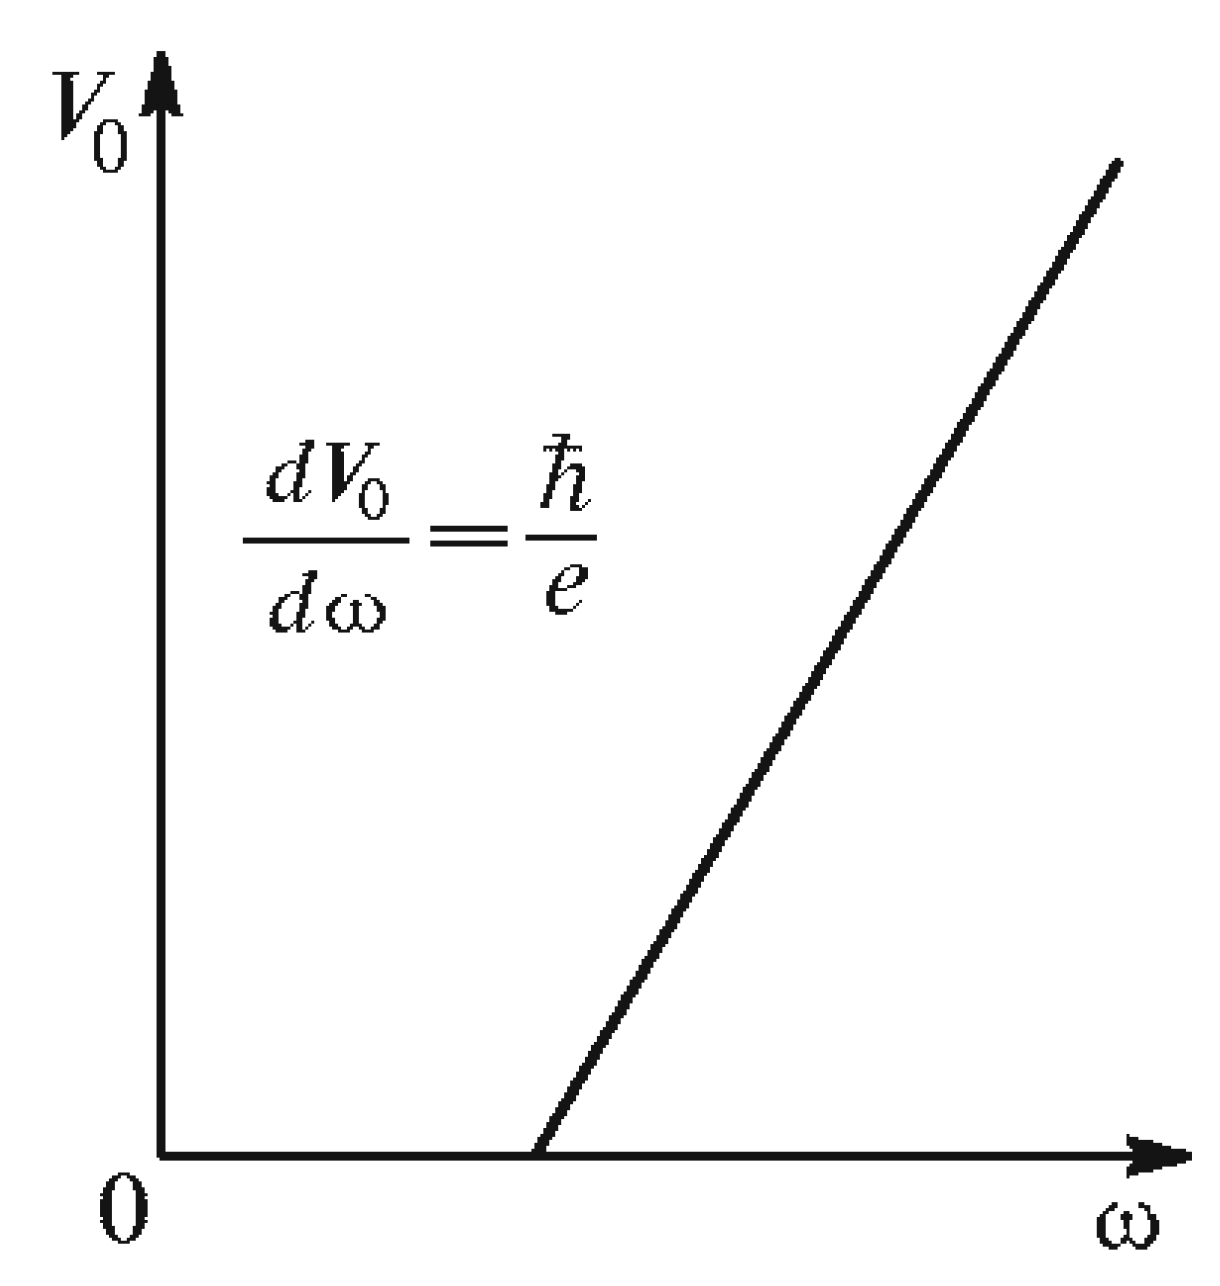
\includegraphics[scale=0.3]{V(w)}
\caption{Зависимость запирающего потенциала
от частоты света}
\label{fig:v_zero}
\end{figure}
	
	Потенциал запирания $ V_0 $ для любого катода линейно зависит от
	частоты света $ \omega $. По наклону прямой на графике $ V_0(\omega) $ (рис. \ref{ris V(w)}) можно определить постоянную Планка:
	
	\begin{equation}\label{e:plank}
	\dfrac{dV_0}{d\omega} = \dfrac{\hbar}{e}
	\end{equation}
	
	Как показывает формула \eqref{dV/dw}, угол наклона прямой $ V_0(\omega) $ не зависит от рода вещества, из которого изготовлен фотокатод. 
\paragraph{Описание установки:}
Принципиальная схема установки представлена на рисунке {\ref{setup}}
\begin{figure}[h!]
\centering
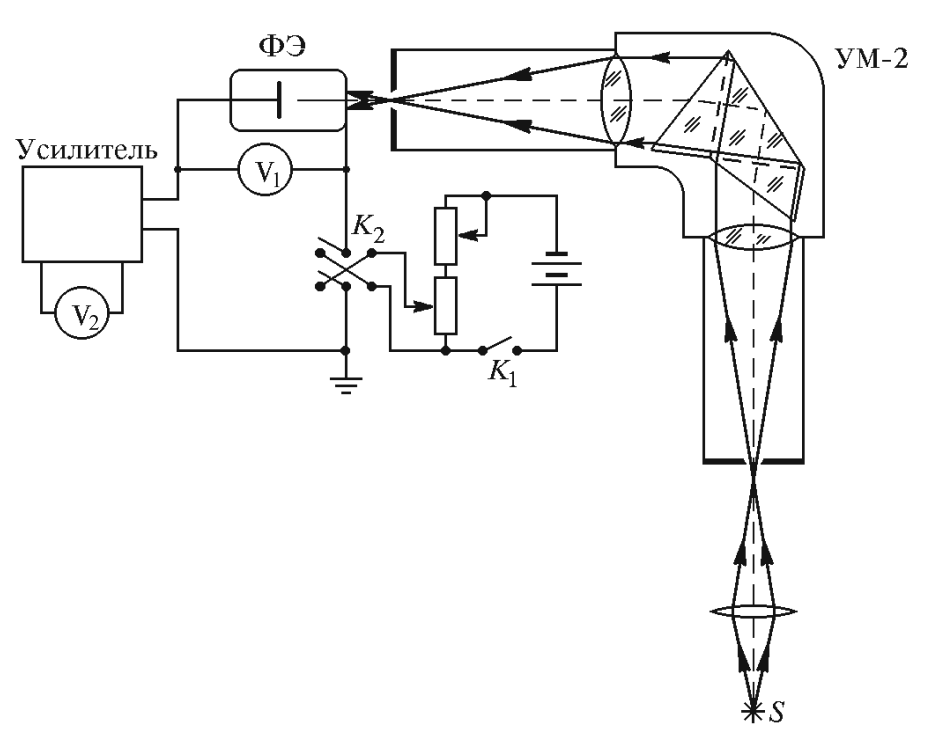
\includegraphics[scale=0.4]{setup.png}
\caption{Принципиальная схема установки}
\label{setup} 
\end{figure}
Установка состоит из:
\begin{enumerate}
\itemsep0em
\item Источника света S (лампа накаливания), свет от которого фокусируется входную на щель с помощью конденсора 
\item Призменного монохроматора УМ-2, выделяющего узкий спектральный интервал
\item Фотоэлемента ФЭ (конструктивно представляет собой откачанный до высокого вакуума стеклянный баллон диаметром 25 мм и высотой 30 мм, внутри которого расположены фотокатод и анод)
\item Усилителя постоянного тока  
\end{enumerate}

\section{Ход работы}

\subsection{Градуировка шкалы монохроматора}

\paragraph{} Поставим в качестве источника света неоновую лампу. Через окуляр будем наблюдать линии спектра неоновой лампы. Измерим показания шкалы монохроматора $\theta$ соответствующие некоторым известным полосам спектра (табл. \ref{tab:calib}).

\begin{table}[h]
\centering
\begin{tabular}{|l|l|l|l|l|l|l|l|l|}
\hline
$N$          & 23      & 22      & 20      & 15      & 13      & 8       & 7       & 1       \\ \hline
$\theta$     & 1880    & 2146    & 2188    & 2266    & 2328    & 2380    & 2428    & 2492    \\ \hline
$\lambda$, Å & 5400.56 & 5852.49 & 5944.83 & 6143.06 & 6217.28 & 6402.24 & 6506.53 & 6717.04 \\ \hline
\end{tabular}
\caption{Номер полосы и соответствующие показание шкалы и длина волны}
\label{tab:calib}
\end{table}

\paragraph{} По данным из табл. \ref{tab:calib} построим калибровочный график, предполагая, что зависимость длины волны $\lambda$ от показания $\theta$ линейная (рис. \ref{fig:calib}).

\begin{figure}[h]
\centering
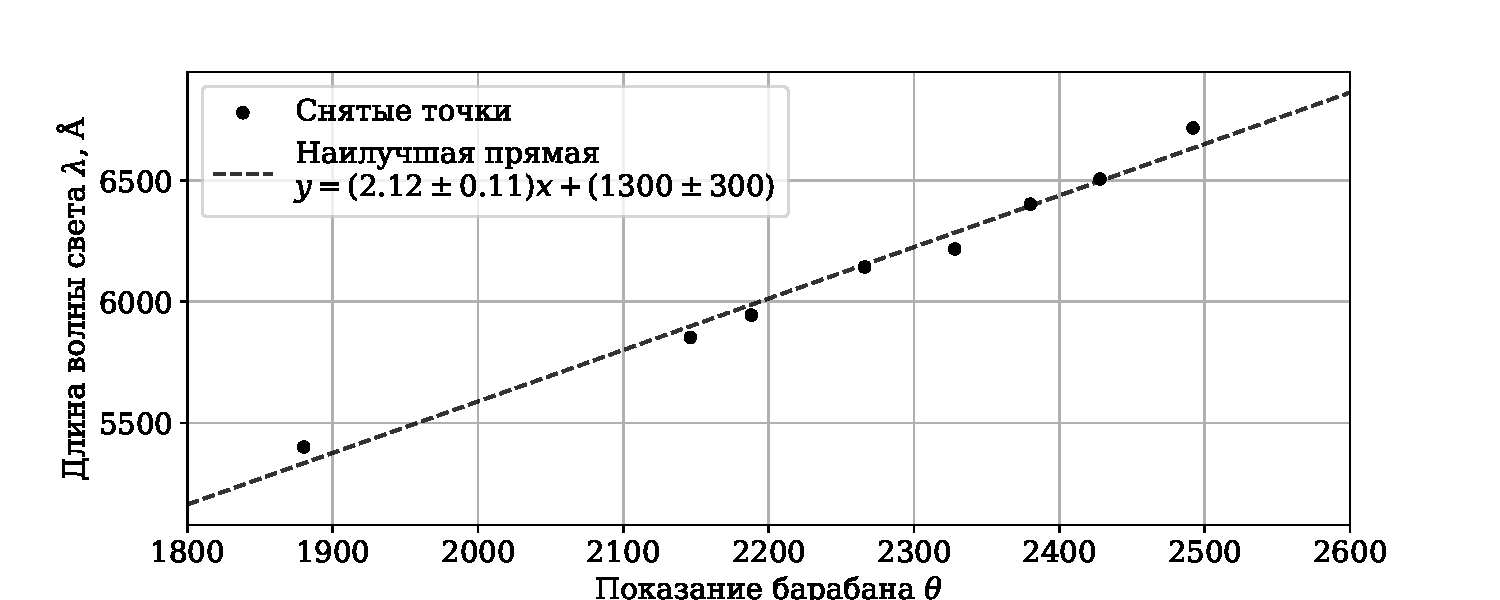
\includegraphics[width=\textwidth]{plot_calib.pdf}
\caption{Калибровочный график $\lambda(\theta)$}
\label{fig:calib}
\end{figure}

\subsection{Снятие вольт-амперной характеристики фотоэлемента}

\paragraph{} Поставим в качестве источника света лампу накаливания. Вместо окуляра поставим фотоэлемент (ФЭ). Для начального измерения выставим монохроматор на зелёный свет ($\theta_1 = 1880$, $\lambda_1 = 5330$ Å). Подберём размеры щелей таким образом, чтобы напряжение на ФЭ не превышало $I \sim 0.6$ В. Меняя тормозящий потенциал $U$ и измеряя напряжение на ФЭ $I$ получим вольт-амперную характеристику фотоэлемента для длины волны $\lambda_1$. Построим график измеренной ВАХ (рис. \ref{fig:general}).

\begin{figure}[h]
\centering
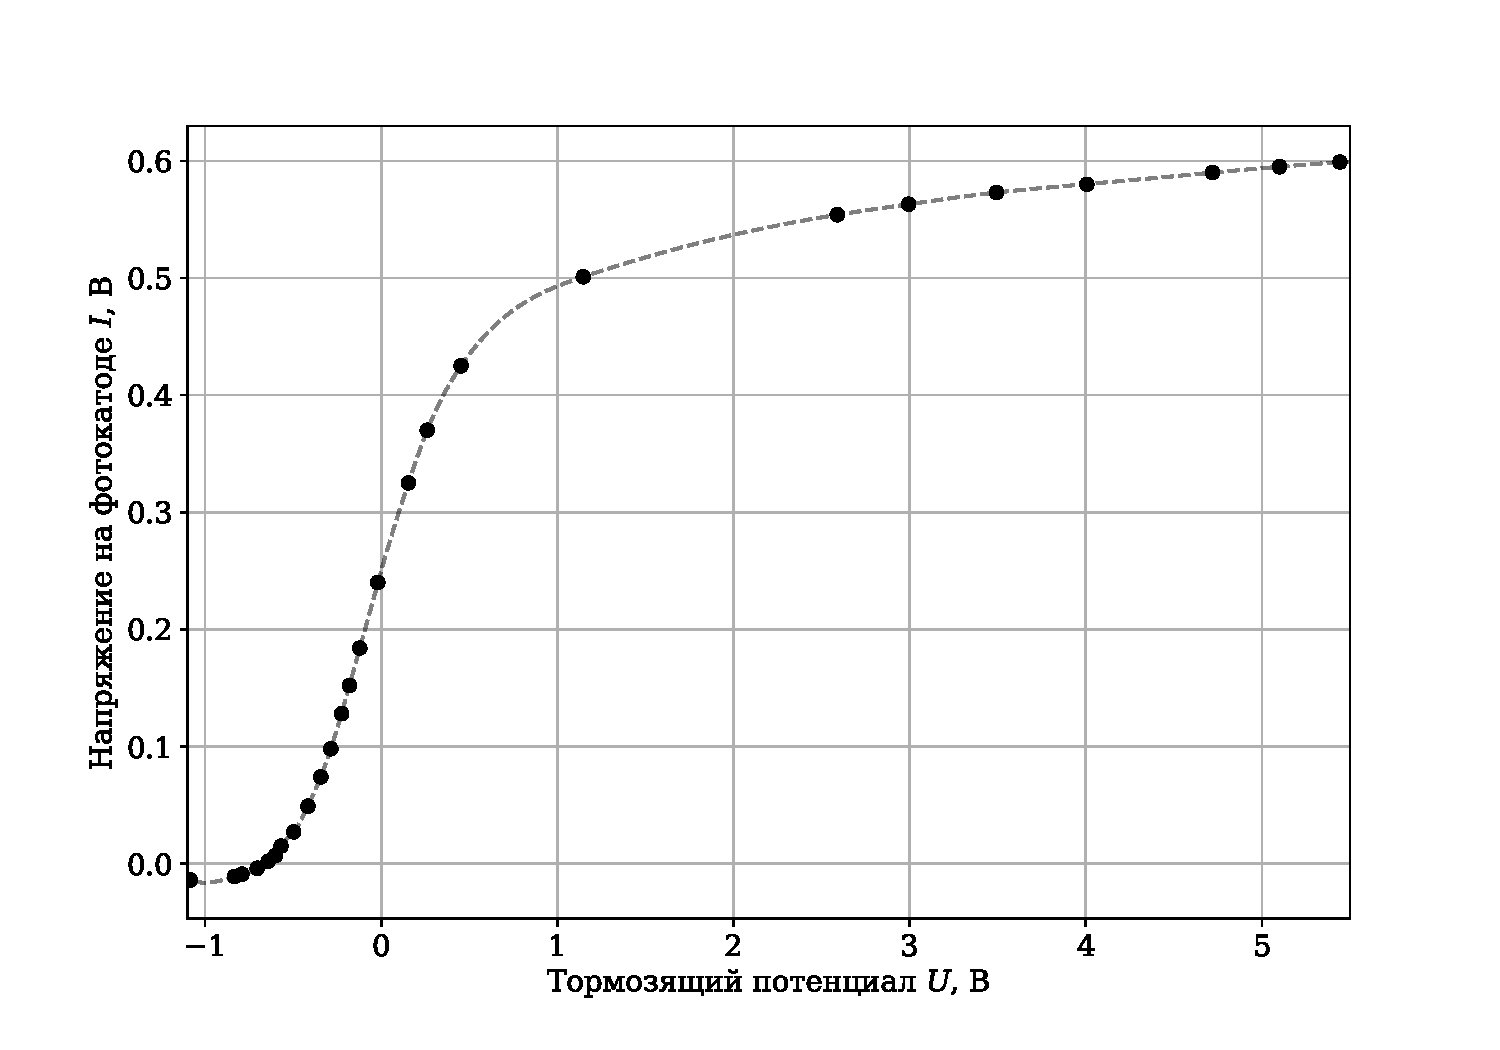
\includegraphics[width=\textwidth]{plot_general.pdf}
\caption{ВАХ ФЭ для длины волны $\lambda_1 = 5330$ Å}
\label{fig:general}
\end{figure}

\paragraph{} Далее измерим ВАХ ФЭ для других длин волн. Снимать ВАХ будем в для отрицательных тормозящих напряжений, так как нас интересует запирающее напряжение. Построим график измеренных ВАХ (рис. \ref{fig:ends}) 

\begin{figure}[h]
\centering
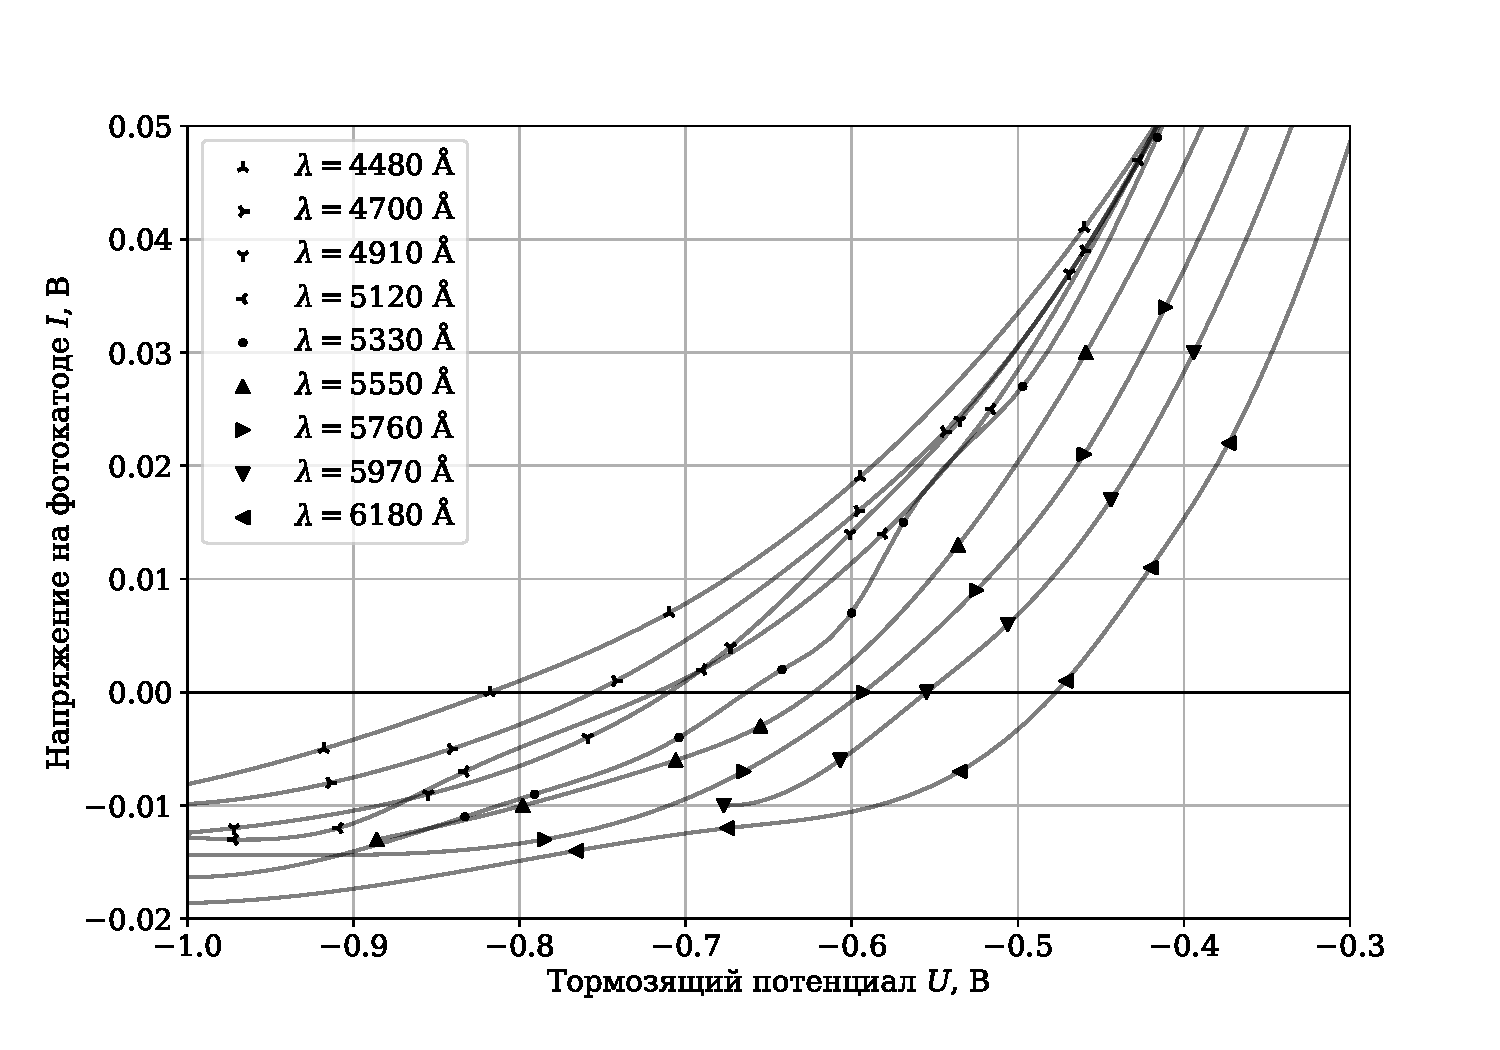
\includegraphics[width=\textwidth]{plot_ends.pdf}
\caption{ВАХ ФЭ для нескольких длин волн}
\label{fig:ends}
\end{figure}

\paragraph{} Пользуясь формулой \eqref{e:i_root} определим по измеренным данным запирающее напряжение для различных длин волн. Для этого построим графики зависимости корня напряжения на ФЭ $\sqrt{I}$ от тормозящего напряжения (рис. \ref{fig:roots}). Графики должны иметь линейный вид. Проведя прямую по методу наименьших квадратов найдём их точки пересечения с осью абсцисс. Точка пересечения прямой $y = ax + b$ с осью абсцисс с погрешностью считается по формуле:

\[
x_0 = - \frac{b}{a}, \;\;\; \Delta x_0 = x_0 \sqrt{\left( \frac{\Delta a}{a} \right) ^ 2 + \left( \frac{\Delta b}{b} \right) ^ 2}.
\]

\noindent Значения для $U_0$ и $\Delta U_0$ для измеренных длин волн запишем в таблицу \ref{tab:u_zeros}.

\begin{figure}[h]
\centering
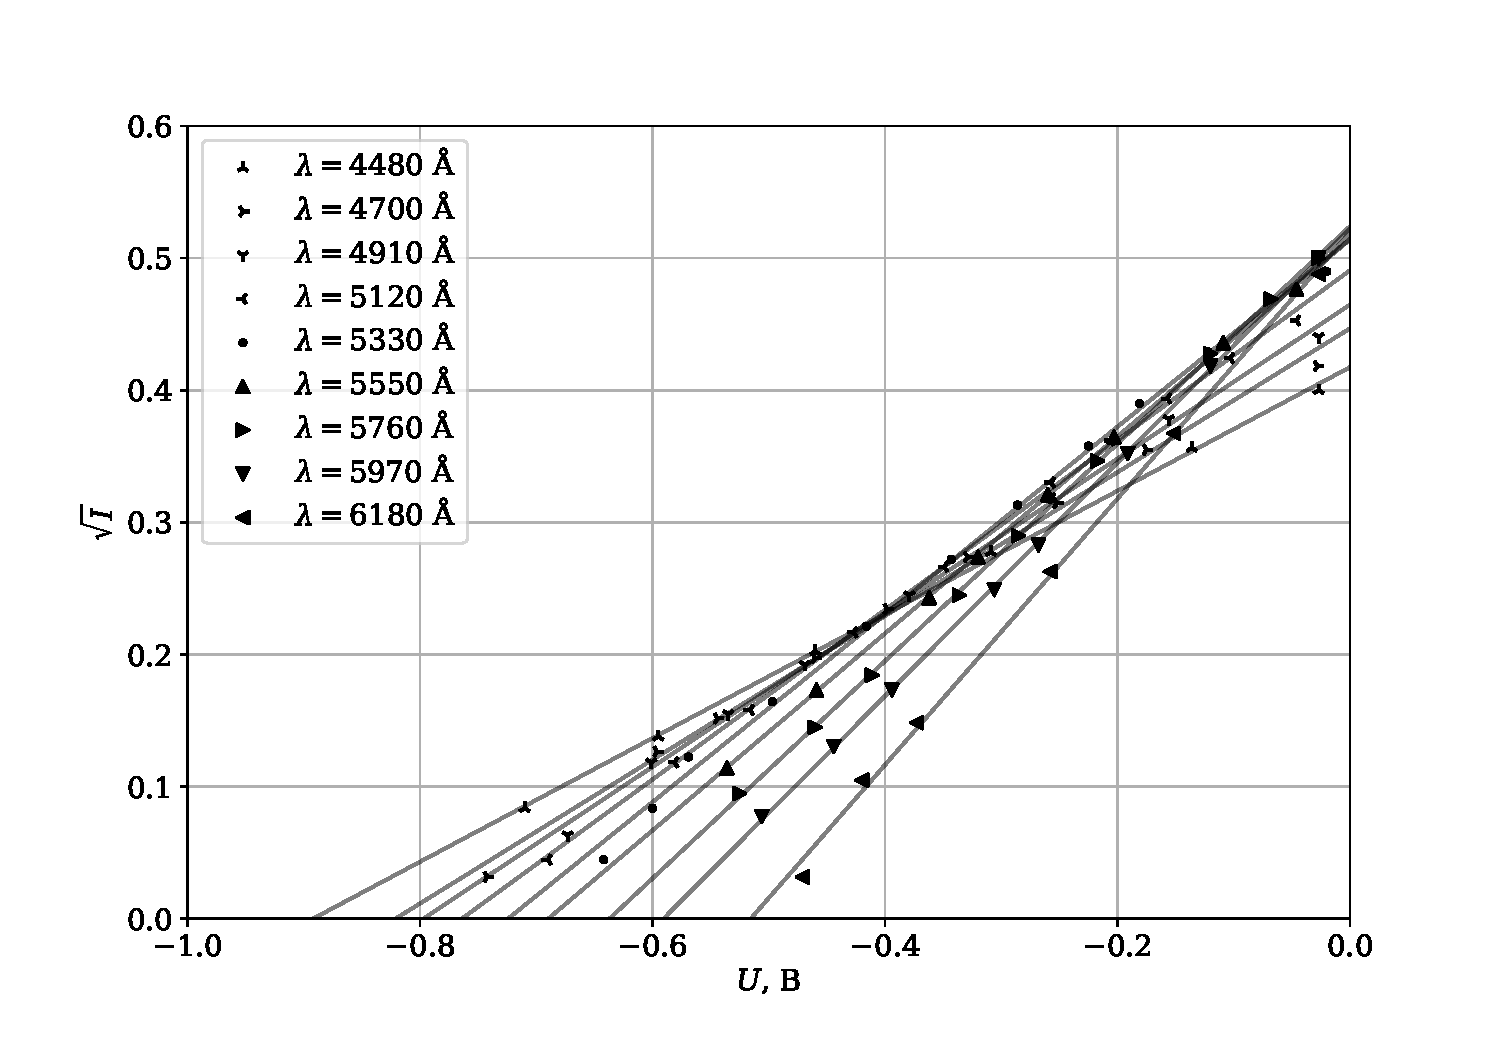
\includegraphics[width=\textwidth]{plot_roots.pdf}
\caption{Зависимость $\sqrt{I}(U)$ и наилучшие прямые}
\label{fig:roots}
\end{figure}

\begin{table}[h]
\centering
\begin{tabular}{|l|l|l|l|l|l|l|l|l|l|}
\hline
$U_0$, В        & 0.89 & 0.82 & 0.80 & 0.764 & 0.72 & 0.69  & 0.637 & 0.591 & 0.52 \\ \hline
$\Delta U_0$, В & 0.01 & 0.02 & 0.02 & 0.008 & 0.01 & 0.005 & 0.003 & 0.004 & 0.02 \\ \hline
$\lambda$, Å    & 4484 & 4696 & 4909 & 5121  & 5334 & 5546  & 5758  & 5971  & 6183 \\ \hline
\end{tabular}
\caption{Значения запирающего напряжения для различных длин волн}
\label{tab:u_zeros}
\end{table}

\subsection{Определение постоянной Планка}

\paragraph{} Построим зависимость измеренных значений запирающего напряжения от круговой частоты света $\omega = 2\pi c/\lambda$, и проведём наилучшею прямую (рис. \ref{fig:plot_plank}). Определим величину постоянной Планка по формуле \eqref{e:plank}:

\[
\hbar = 3.1 \cdot 10^{-16} \cdot e = 3.1 \cdot 10^{-16} \cdot 1.6 \cdot 10^{-19} = 5.0 \cdot 10^{-35} \; \text{Дж} \cdot \text{с},
\]\[
\Delta \hbar = 0.2 \cdot 10^{-16} \cdot e = 0.3 \cdot 10^{-35} \; \text{Дж} \cdot \text{с}.
\]

\noindent Получили значение $\hbar = (0.50 \pm 0.03) \cdot 10^{-34}$ Дж$\cdot$с.

\begin{figure}[h]
\centering
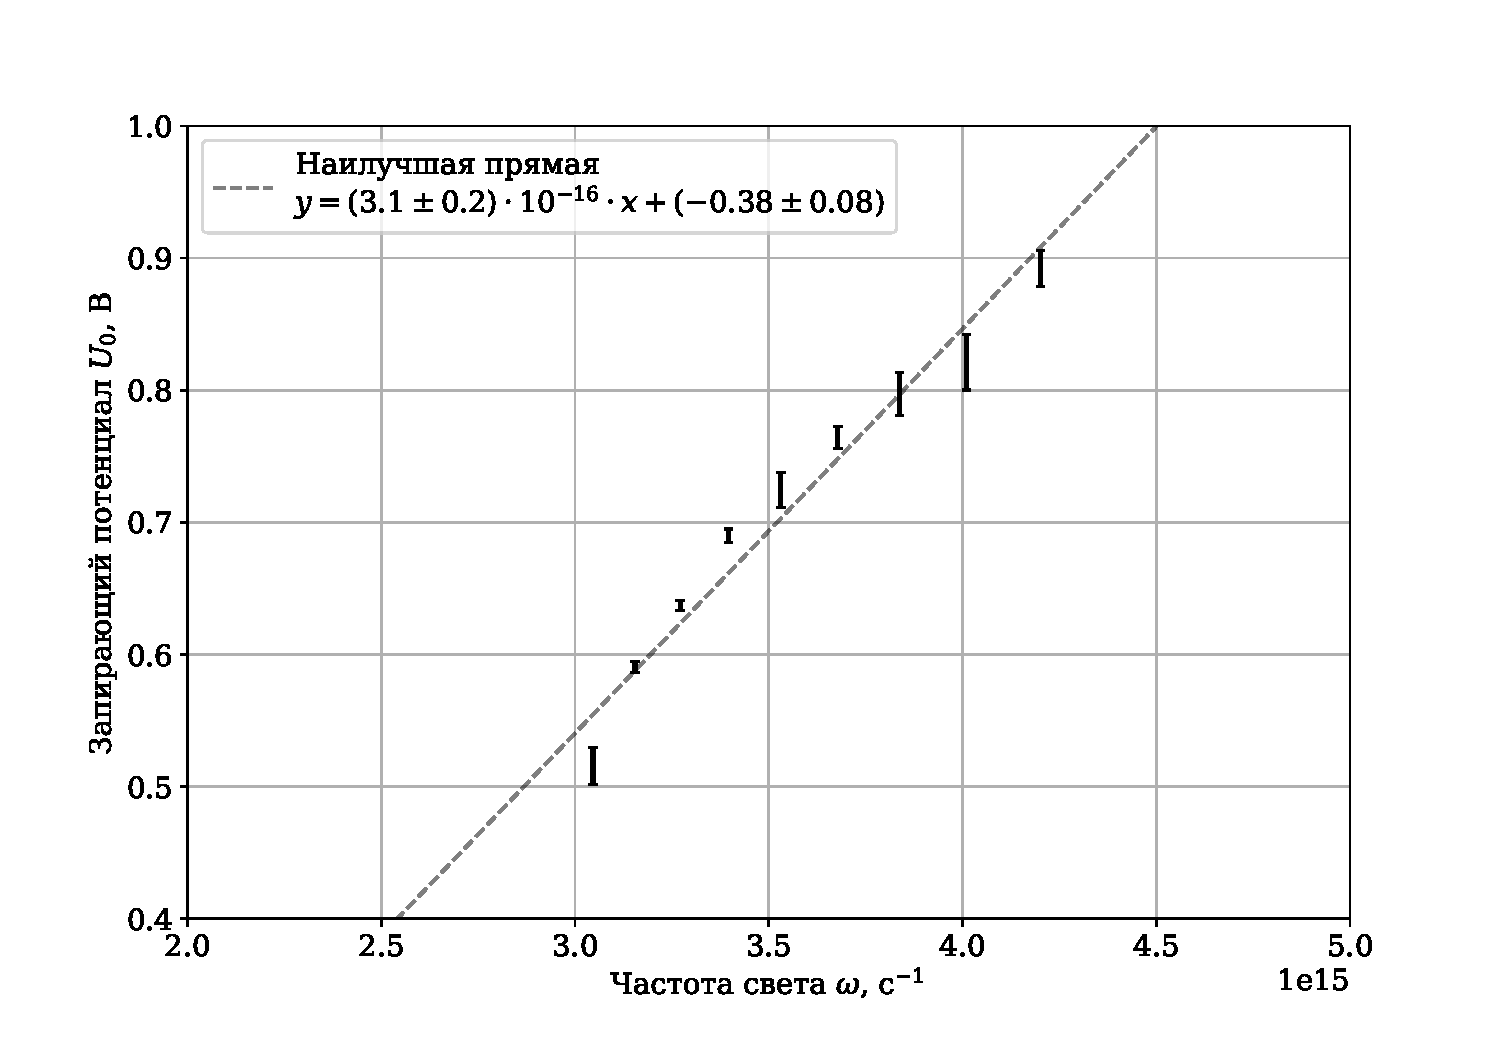
\includegraphics[width=\textwidth]{plot_plank.pdf}
\caption{Зависимость $U_0(\omega)$ и наилучшая прямая}
\label{fig:plot_plank}
\end{figure}


\section{Выводы}
\begin{enumerate}
\item Пронаблюдали фотоэффект, и получили вольт-амперную характеристику соответствующую теоретической.
\item Подтвердили уравнение Эйнштейна для фотоэффекта, показав, что запирающее напряжение пропорционально частоте света.
\item Получили оценку постоянной планка $\hbar = (0.50 \pm 0.03) \cdot 10^{-34}$ Дж$\cdot$с, что примерно в два раза меньше действительного значения $\hbar = 1.0545 \cdot 10^{-34}$ Дж$\cdot$с. Полученное значение может быть улучшено, если снять более точный калибровочный график, который учитывает нелинейность шкалы монохроматора.
\end{enumerate}
\end{document}